\documentclass[UTF-8]{article}


\usepackage{booktabs}
\usepackage{url}
\usepackage{cite}
\usepackage[version=4]{mhchem}
\usepackage{graphicx}
\usepackage{subfigure}
\usepackage[a4paper,top=2cm,bottom=2cm,right=3cm,left=3cm,marginparwidth=1.75cm]{geometry}
\usepackage{amsmath}
\usepackage{upgreek}

\title{Template}
\author{Yan Haoming}
\date{September 27, 2024}


\begin{document}
\maketitle
\begin{abstract}
    pass now.
\end{abstract}
\textbf{Keywords: }
\section{Theory}
\subsection{Meaning of Symbols}
To emphasis the time dependence of some variables, I add subscript to them, which is slightly different from the original article.
\begin{itemize}
    \item $C$: number of similar \textbf{cultures} in our experiment.
    \item $t$: time in units of division cycles of the yeasts.
    \begin{itemize}
        \item thus the growth rate should be exactly 1, both for sensitive yeasts and resistant yeasts.
        \item $t_0$: a certain time, prior to which mutations were not likely to occur in any experimental \textbf{cultures}.
        Specifically speaking the $t_0$ satisfies:
        $$
        1=\text{Ex}(Cm_{t_0}))=\text{Ex}(aC(N_{t_0}-N_0))
        $$
    \end{itemize}
    \item $N_t$, \textit{observable}: number of yeasts in \textbf{a growing culture} at time $t$.
    \begin{itemize}
        \item $N_t-N_0$: increase in the number of yeasts.
        \item $N_0\ll N_t$, thus, $N_0\approx 0$ in the presence of $N_t$.
    \end{itemize}
    \item $\rho _t$: the \textbf{average} number of resistant yeasts present at time $t$, in one \textbf{culture}.
    \item $r_t$, \textit{observable}: the \textbf{likely average} number of resistant yeasts in a \textbf{culture} at time $t$, gotten from \textbf{limited number of samples}.
    \item $a$: mutation rate, namely, the chance of mutation per yeast per time unit.
    \item $m_t$: the \textbf{average} number of mutations at time $t$, in \textbf{a culture}.
    \item $p_0$: the fraction of cultures showing \textbf{no} mutation in a large series of similar cultures.


\end{itemize}
\subsection{Derivation of the Formulas}
\subsubsection{Acquired Hereditary Immunity Hypothesis}
\textit{Assumption: a fixed small chance for each yeast to survive an attack.}
\begin{align}
    \text{Number of resistant yeasts}&\sim\text{Binomial Distribution}\\
    &\sim\text{Poisson Distribution}
\end{align}
\begin{align}
    \text{Var}(r_t)&=\text{Ex}(r_t)=r_t\\
\end{align}

\subsubsection{Mutation Hypothesis}
\textit{Assumption: a fixed small chance per time unit for each yeast to undergo a mutation to resistance.}
\begin{align}
    \frac{dN_t}{dt}&=N_t\\
    N_t &=N_0e^t\\
    dm_t &=a dt N_t\\
    m_t &=a(N_t-N_0)
\end{align}
\begin{align}
    \text{Number of yeasts mutate during }dt&\sim\text{Poisson Distribution}
\end{align}
\begin{align}
    p_0&=e^{-m_t}\\
    \frac{d \rho _t}{dt}&=aN_t+\rho\\
    \text{assume: }\rho_0&=0\\
    \rho_t&=taN_t\\
    r_t&=(t-t_0)aN_t\\
    1&=aC(N_{t_0}-N_0)\approx aCN_{t_0}\\
    N_{t_0}&=N_te^{-(t-t_0)}\\
    t-t_0&=\ln(N_tCa)\\
    r_t&=aN_t\ln(N_tCa)
\end{align}
The following discussion is about \textbf{partial distribution}, defined as the distribution during a certain time interval from $t-\tau$ to $t-\tau+d\tau$ with $t$ fixed while $\tau$ as parameter:
\begin{align}
    \text{Ex}(dm_t)&=aN_{\tau}d\tau =aN_te^{-\tau}d \tau\\
    d\rho_t&=e^{\tau}dm_t\\
    \text{Ex}(d\rho_t)&=e^{\tau}\text{Ex}(dm_t)=aN_td\tau\\
    \text{Var}(d{\rho_t})&=e^{2\tau}\text{Var}(dm_t)=aN_te^{\tau}d\tau\\
\end{align}
To find the total distribution from partial distribution:
\begin{align}
    \text{Var}({\rho_t})&=\int_{0}^{t}\text{Var}({d\rho_t})d\tau\\
    &=aN_t(e^t-1)\\
    \text{Var}({r_t})&=\int_{0}^{t-t_0}\text{Var}({dr_t})d\tau\\
    &=aN_t(e^{t-t_0}-1)\\
    &\approx Ca^2N_t^2\\
    \frac{\text{Var}(r_t)}{r_t}&=\frac{CaN_t}{\ln(N_tCa)}\gg 1
\end{align}
\section{Calculating Procedure in Experiment}
\begin{itemize}
    \item observe the number of yeasts in a growing culture $N_t$ at time $t$.
    \item determine the number of resistant yeasts in each \textbf{sample}.
    \begin{itemize}
        \item this should be carried out by observing the number of colonies several days after inoculating.
    \end{itemize}
    \item calculate the number of resistant yeasts $r_t$ in each \textbf{culture}:
    $$
    r_t=\frac{\text{volume of culture}}{\text{volume of samples}}\cdot \text{Ex}(r_{t\text{ sample}})
    $$
    \begin{itemize}
        \item $\text{volume of culture}=1$ mL, $\text{volume of samples}=20\ \upmu $L in our experiment.
    \end{itemize}
    \item evaluate the mutation rate $a$ by the following formula:
    $$
    r_t=aN_t\ln(N_tCa)
    $$
    \item figure out the likely variance $\text{Var}(r_t)$:
    \begin{itemize}
        \item by mutation rate $a$ according to the theory:
        $$
        \text{Var}({r_t})\approx Ca^2N_t^2
        $$
        \item by statistical methods:
        
        $$
        \text{Var}(\tilde{r_{t \text{ sample}}})=\text{Var}(r_{t \text{ sample}})-\text{Var}(\text{sampling})
        $$

        $$
        \text{Var}(\text{sampling})\approx\text{Ex}(\text{sampling})=r_t
        $$
        $$
        \text{Var}({r_t})=\left( \frac{\text{volume of culture}}{\text{volume of samples}} \right)^2\cdot\text{Var}(\tilde{r_{t \text{ sample}}}) 
        $$
        Thus we calculate the modified statistical variance by:
        $$
        \text{Var}({r_t})=\left( \frac{\text{volume of culture}}{\text{volume of samples}} \right)^2\cdot(\text{Var}(r_{t \text{ sample}}) -\text{Ex}(r_{t \text{ sample}}))
        $$
        \item compare the ratio of variance and average to one (Poisson distribution in Acquired hereditary immunity hypothesis):
        $$
        \frac{\text{Var}(r_t)}{\text{Ex}(r_t)}
        $$
        both by the statistical method (just based on the final result) and by the theoretical method (based on the mutation rate $a$).
    \end{itemize}


\end{itemize}













\section{Part One}
This is a template for convenient writing process.
The text book helps\cite{TheCell} me a lot.
We should use bibtex to compile the document,


$\upmu\mathrm{m}$

$\mathrm{\mu}=12345$

 % Figure
 \begin{figure}
    \centering
    \subfigure[fig 1]{
\includegraphics[width=0.7\linewidth]{../Figures/example 1.png}}
    \subfigure[fig 2]{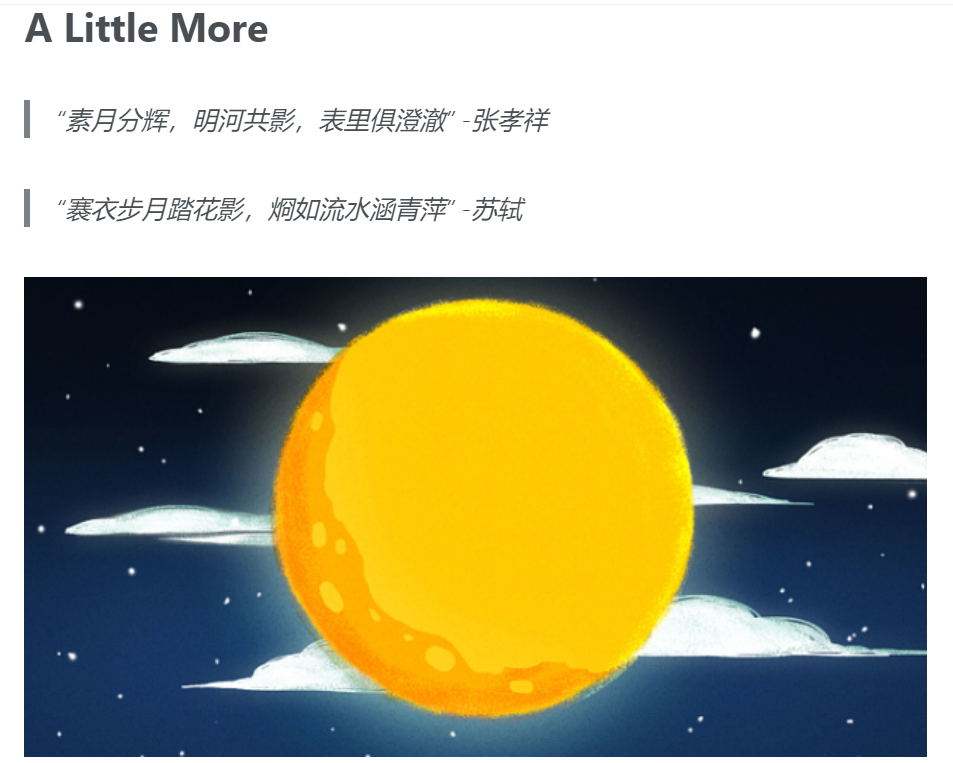
\includegraphics[width=0.7\linewidth]{../Figures/example 2.png}}
    \caption{example 1}  
    \label{example 1}
 \end{figure}

\begin{figure}
    \centering
    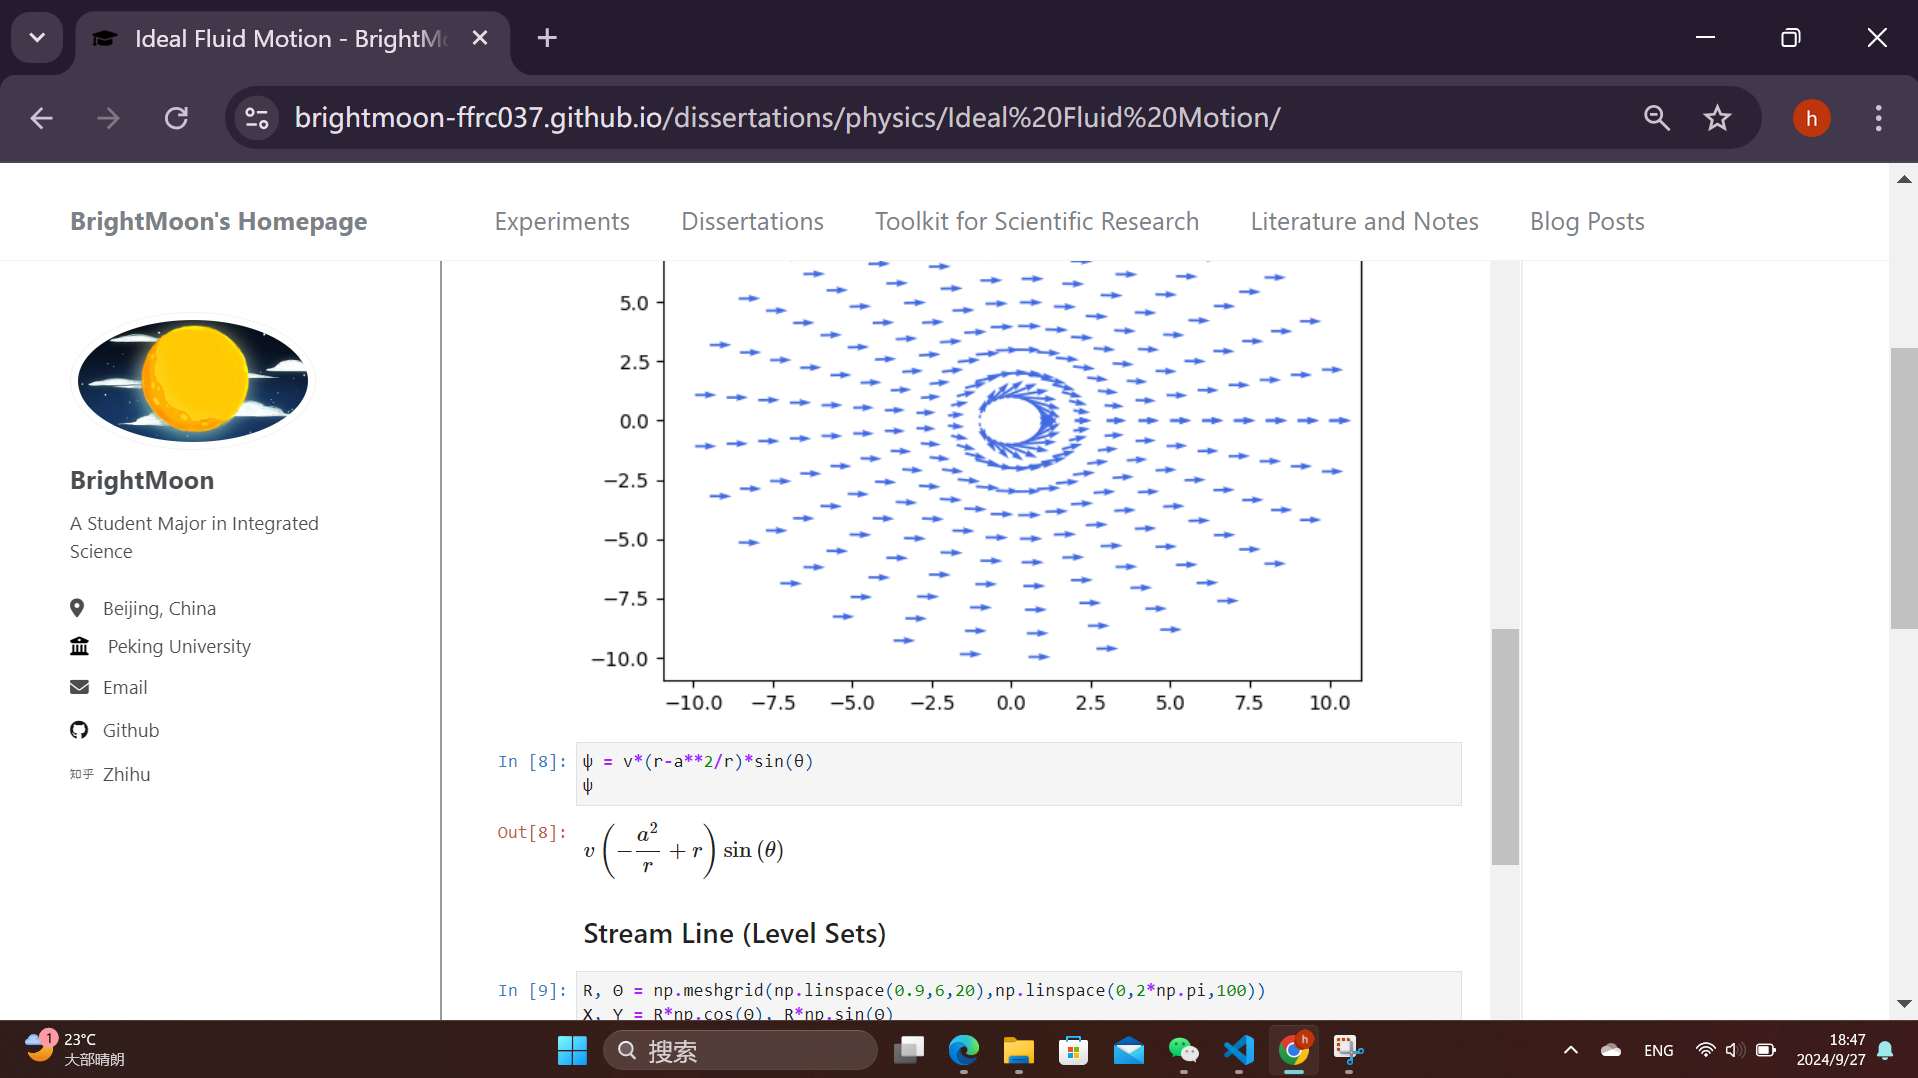
\includegraphics[width=0.7\linewidth]{../Figures/example 3.png}
    \caption{example 2}
    \label{example 2}
\end{figure}

% Table
\begin{table}
    \centering
    \begin{tabular}{|c|c|}\hline
        Column One & Column Two \\ \hline
        Content One & Content One\\ \hline
    \end{tabular}
    \caption{example 3}
    \label{example 3}
\end{table}

% List
\begin{itemize}
    \item item 1
    \item item 2
\end{itemize}


\bibliographystyle{plain}
\bibliography{references}
\end{document}